% Options for packages loaded elsewhere
\PassOptionsToPackage{unicode}{hyperref}
\PassOptionsToPackage{hyphens}{url}
%
\documentclass[
]{article}
\usepackage{amsmath,amssymb}
\usepackage{lmodern}
\usepackage{iftex}
\ifPDFTeX
  \usepackage[T1]{fontenc}
  \usepackage[utf8]{inputenc}
  \usepackage{textcomp} % provide euro and other symbols
\else % if luatex or xetex
  \usepackage{unicode-math}
  \defaultfontfeatures{Scale=MatchLowercase}
  \defaultfontfeatures[\rmfamily]{Ligatures=TeX,Scale=1}
\fi
% Use upquote if available, for straight quotes in verbatim environments
\IfFileExists{upquote.sty}{\usepackage{upquote}}{}
\IfFileExists{microtype.sty}{% use microtype if available
  \usepackage[]{microtype}
  \UseMicrotypeSet[protrusion]{basicmath} % disable protrusion for tt fonts
}{}
\makeatletter
\@ifundefined{KOMAClassName}{% if non-KOMA class
  \IfFileExists{parskip.sty}{%
    \usepackage{parskip}
  }{% else
    \setlength{\parindent}{0pt}
    \setlength{\parskip}{6pt plus 2pt minus 1pt}}
}{% if KOMA class
  \KOMAoptions{parskip=half}}
\makeatother
\usepackage{xcolor}
\IfFileExists{xurl.sty}{\usepackage{xurl}}{} % add URL line breaks if available
\IfFileExists{bookmark.sty}{\usepackage{bookmark}}{\usepackage{hyperref}}
\hypersetup{
  pdftitle={Project Fisheries - FRB Cesab training},
  pdfauthor={Céline Albert, Samuel Charberet, Lola Gilbert},
  hidelinks,
  pdfcreator={LaTeX via pandoc}}
\urlstyle{same} % disable monospaced font for URLs
\usepackage[margin=1in]{geometry}
\usepackage{graphicx}
\makeatletter
\def\maxwidth{\ifdim\Gin@nat@width>\linewidth\linewidth\else\Gin@nat@width\fi}
\def\maxheight{\ifdim\Gin@nat@height>\textheight\textheight\else\Gin@nat@height\fi}
\makeatother
% Scale images if necessary, so that they will not overflow the page
% margins by default, and it is still possible to overwrite the defaults
% using explicit options in \includegraphics[width, height, ...]{}
\setkeys{Gin}{width=\maxwidth,height=\maxheight,keepaspectratio}
% Set default figure placement to htbp
\makeatletter
\def\fps@figure{htbp}
\makeatother
\setlength{\emergencystretch}{3em} % prevent overfull lines
\providecommand{\tightlist}{%
  \setlength{\itemsep}{0pt}\setlength{\parskip}{0pt}}
\setcounter{secnumdepth}{-\maxdimen} % remove section numbering
\ifLuaTeX
  \usepackage{selnolig}  % disable illegal ligatures
\fi

\title{\textbf{Project Fisheries - FRB Cesab training}}
\author{Céline \textbf{Albert}, Samuel \textbf{Charberet}, Lola
\textbf{Gilbert}}
\date{02/12/2021}

\begin{document}
\maketitle

The project is available on
\emph{\href{https://github.com/samuelcharberet/project.frb.fisheries}{github}}

\hypertarget{r-work-environment}{%
\subsection{1. R work environment}\label{r-work-environment}}

For this project we used:

\begin{itemize}
\tightlist
\item
  Targets to manage our workflow
\item
  renv to make our R environment reproducible
\item
  Rmarkdown to generate both this presentation and a Latex report
\item
  ggplot2 to visualize our data
\end{itemize}

\hypertarget{data}{%
\subsection{2. Data}\label{data}}

\hypertarget{data-extracted}{%
\subsection{\#\#\# 2.1. Data extracted}\label{data-extracted}}

\begin{itemize}
\item ~
  \hypertarget{carbone-c-nitrogen-n-phosphorus-p-content-of-dry-mass-from-jabot-f.-et-al.-2020-dataset-for-the-article-body-stoichiometry-of-heterotrophs-assessing-drivers-of-interspecific-variations-in-elemental-composition.-figshare.-dataset.-httpsdoi.org10.6084m9.figshare.13366310.v1}{%
  \subsection{\texorpdfstring{\textbf{Carbone (C), Nitrogen (N),
  Phosphorus (P)} content (\% of dry mass) from Jabot, F. et al.,
  (2020): Dataset for the article ``Body stoichiometry of heterotrophs:
  assessing drivers of interspecific variations in elemental
  composition''. figshare. Dataset.
  \url{https://doi.org/10.6084/m9.figshare.13366310.v1}}{Carbone (C), Nitrogen (N), Phosphorus (P) content (\% of dry mass) from Jabot, F. et al., (2020): Dataset for the article ``Body stoichiometry of heterotrophs: assessing drivers of interspecific variations in elemental composition''. figshare. Dataset. https://doi.org/10.6084/m9.figshare.13366310.v1}}\label{carbone-c-nitrogen-n-phosphorus-p-content-of-dry-mass-from-jabot-f.-et-al.-2020-dataset-for-the-article-body-stoichiometry-of-heterotrophs-assessing-drivers-of-interspecific-variations-in-elemental-composition.-figshare.-dataset.-httpsdoi.org10.6084m9.figshare.13366310.v1}}
\item
  \textbf{Tonnage} from \emph{Sea Around Us} We downloaded data for the
  Barents Sea area on the Website: \url{https://www.seaaroundus.org/}
\item
  \textbf{Taxonomic data} from the Global Biodiveristy Information
  Facility (GBIF)
\end{itemize}

\hypertarget{data-manipulation}{%
\subsubsection{2.2. Data manipulation}\label{data-manipulation}}

Having two different dataset has required to join them. However, the
species name were not exactly noted the same way on the two documents.
Therefore we had to do some cleaning/filetering on both datasets.

\hypertarget{final-dataset}{%
\subsubsection{2.3. Final dataset}\label{final-dataset}}

Our final dataset contains:\\
* Carbone (C)\\
* Nitrogen (N)\\
* Phosphorus (P)\\
* Species (n species of fishes)\\
* Tonnage\\
* Countries\\
* Type of gear

\hypertarget{analyses-and-vizualisation}{%
\subsection{3. Analyses and
vizualisation}\label{analyses-and-vizualisation}}

\hypertarget{representation-of}{%
\subsubsection{Representation of \ldots{}}\label{representation-of}}

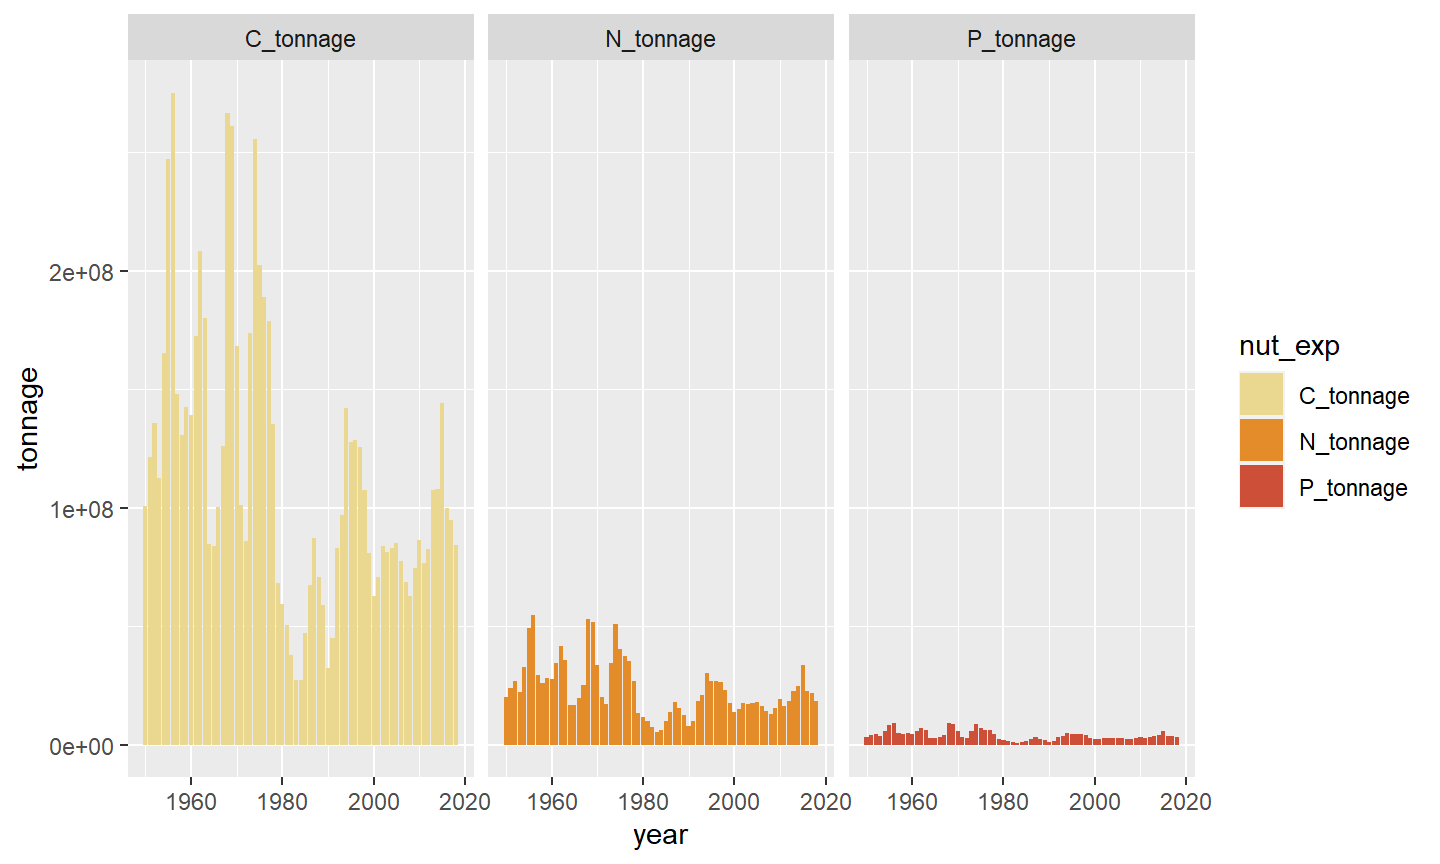
\includegraphics{ProjectFisheries_files/figure-latex/unnamed-chunk-1-1.pdf}

\hypertarget{bibliography}{%
\subsection{4. Bibliography}\label{bibliography}}

\end{document}
